\section{Задание 1}

Произвести ликвидацию перегрузки ресурсов в проекте

Microsoft Project показывает перегрузку следующих ресурсов:
\begin{enumerate}
	\item Системный аналитик:
	\begin{enumerate}
		\item Анализ и построение структуры базы объектов;
		\item Анализ и проектирование ядра.
	\end{enumerate}
	\item Художник-дизайнер
	\begin{enumerate}
		\item Разработка дизайна руководства;
		\item Разработка дизайна сайта.
	\end{enumerate}
	\item Технический писатель:
	\begin{enumerate}
		\item Написание руководства пользователя;
		\item Создание справочной системы.
	\end{enumerate}
\end{enumerate}

Перегрузку ресурсов можно устранить несколькими способами:
\begin{enumerate}
	\item изменить календарь работы ресурса;
	\item назначить ресурс на неполный рабочий день;
	\item изменить профиль назначения ресурса;
	\item изменить ставку оплаты ресурса;
	\item добавить ресурсу время задерки;
	\item разбить задачу на этапы и перекрыть по времени их выполнения;
	\item автоматическое выравниевание;
\end{enumerate}

Проведем автоматическое выравнивание ресурсов. Используем следующие настройки выравнивания (См. рисунок \ref{fig:lab311})

\begin{figure}[H]
	\centering
	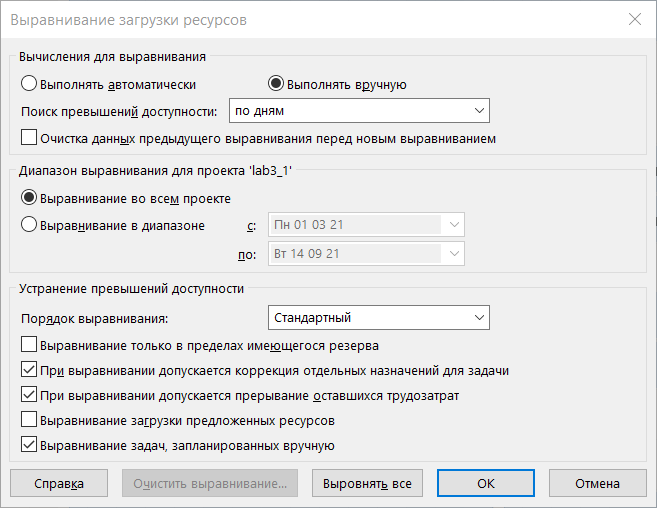
\includegraphics[width=0.7\linewidth]{../../lab_03/report/src/lab3_1_1}
	\caption{Настройки выравнивания ресурсов.}
	\label{fig:lab311}
\end{figure}

После авто выравнивания перегрузка ресурсов ушла, но увеличились затраты (С 47500 до 47902).
И продолжительсность проекта возросла до 28 недели, что не удовлетворяет условиям.

\section{Задание 2}
Подзадачи:
\begin{enumerate}
	\item Отразите в плане проекта проведение еженедельного совещания по
	средам с 10 до 11 утра;
	\item Привлеките к участию в совещании всех специалистов, кроме
	наборщиков данных и программистов №1 - 4 (их интересы на совещании
	представляет ведущий программист).
	\item Устраните перегрузку ресурсов.
	\item В случае превышения бюджета и сроков реализации проекта проведите
	оптимизацию временных и финансовых параметров проекта.
\end{enumerate}

После добавления еженедельного совещания появились следующие проблемы:
\begin{enumerate}
	\item Стоимость проекта увеличилась с 47902р до 67941р. Стоимость проекта увеличилась на 20039р
	\item Появилась перегрузка ресурсов, что логично, по скольку сотрудник не может выполнять задачу и находится на совещании.
\end{enumerate}

Очевидным решением является уменьшение заработной платы на время совещания.
Для всех ресурсов задействованных на совещании поменяем составим дополнительные ставки (см рисунок \ref{fig:lab321}).

\begin{figure}[H]
	\centering
	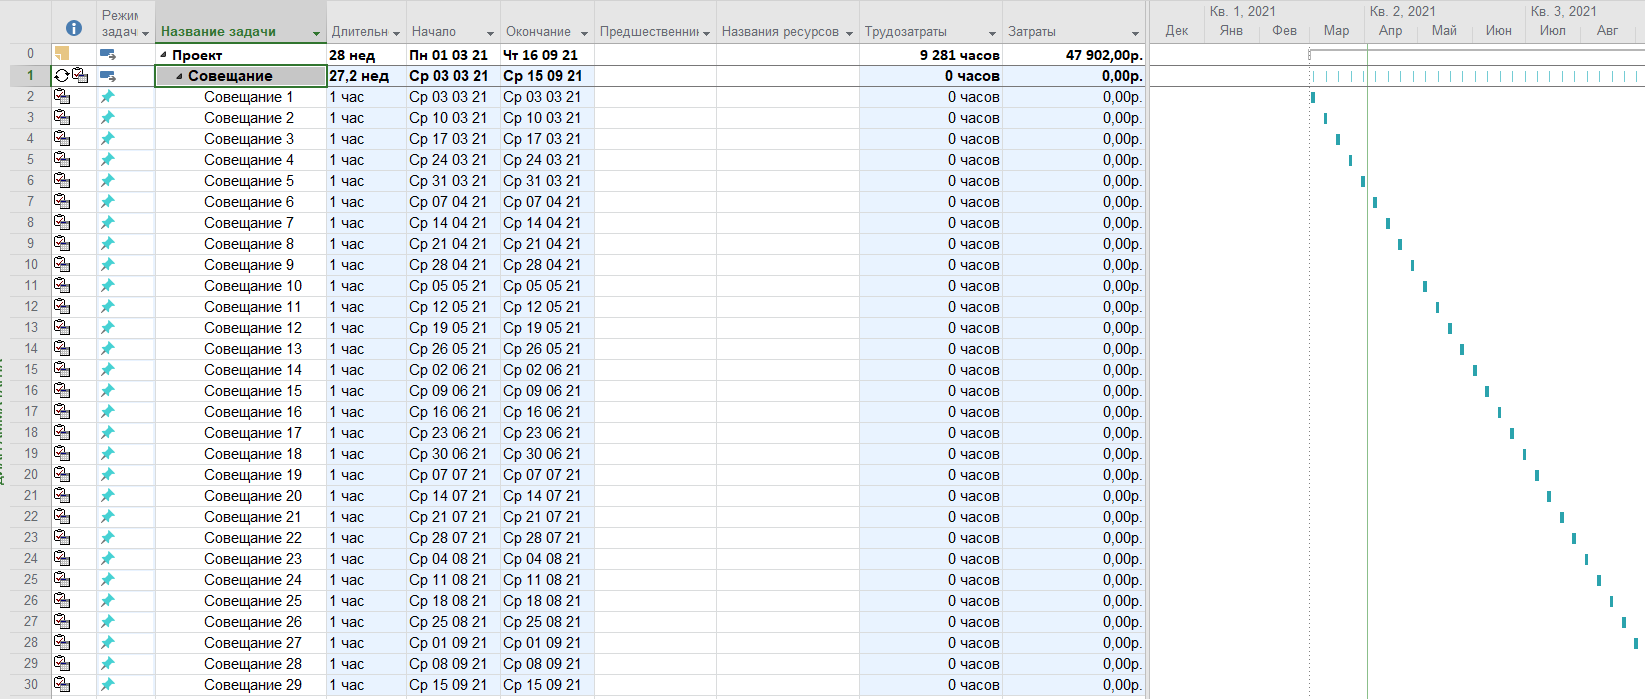
\includegraphics[width=0.7\linewidth]{../../lab_03/report/src/lab3_2_1}
	\caption{Пониженная ставка}
	\label{fig:lab321}
\end{figure}


















